\chapter{Processor Architecture}

\section{Fixed-Program Computer}

A \textbf{fixed-program computer} is a computer that is designed for a particular task. Reprogramming a fixed-program computer may not be possible, or might require restructuring or re-wiring the machine.

\subsection{ENIAC}



\section{Stored-Program Computer}



\section{Von Neumann Architecture}

\subsection{History}

The original description of a von Neumann architecture defines a computer as having the following components:

\begin{itemize}
	\item Processing unit (ALU + processor registers)
	\item Control unit (PC + instruction registers)
	\item Memory
	\item External mass storage
	\item Input and output mechanisms
\end{itemize}

\subsection{Definition}

\begin{figure}[h!]
	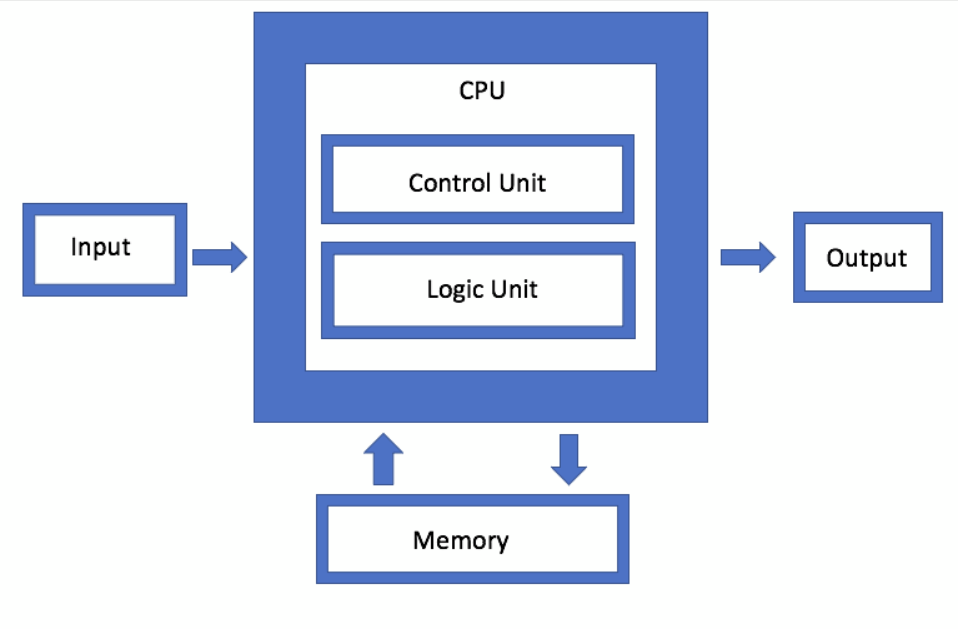
\includegraphics[scale=0.5]{./img/von-Neumann.png}
\end{figure}

A von Neumann architecture generally describes a stored-program computer with a shared memory for data and instructions. Instructions are executed sequentially. The computer fetches one instruction at a time from memory and sends it to the CPU.

\subsection{Von Neumann Bottleneck}

The \textbf{von Neumann bottleneck} is the reduction in throughput caused by the single bus, which can only access data or instruction data at once.

\subsection{Self-Modifying Code}

In the von Neumann architecture, there is no distinction between data and instruction data. 

\section{Harvard Architecture}

The \textbf{Harvard architecture} is a variant of the von Neumann architecture that attempts to address its limitations. It has separate memories for data and instructions, and separate connections between each and the central control.

This means that the instruction memory can be implemented in ROM, and have a different word length than the data memory, since the two memories utilize different buses that may be of different widths.

Applications that commonly use the Harvard architecture include DSP (digital signal processing) applications and microprocessors.

\section{References}

\begin{itemize}
	\item Computer Systems a Programmer's Perspective
	\item https://ftp.arl.army.mil/~mike/comphist/eniac-story.html
	\item Arikpo, I., Ogban, F. U. \& Eteng, I., E. (2007) Von Neumann architecture and modern computers
\end{itemize}